% Options for packages loaded elsewhere
\PassOptionsToPackage{unicode}{hyperref}
\PassOptionsToPackage{hyphens}{url}
\PassOptionsToPackage{dvipsnames,svgnames,x11names}{xcolor}
%
\documentclass[
  10pt,
]{article}
\usepackage{amsmath,amssymb}
\usepackage{iftex}
\ifPDFTeX
  \usepackage[T1]{fontenc}
  \usepackage[utf8]{inputenc}
  \usepackage{textcomp} % provide euro and other symbols
\else % if luatex or xetex
  \usepackage{unicode-math} % this also loads fontspec
  \defaultfontfeatures{Scale=MatchLowercase}
  \defaultfontfeatures[\rmfamily]{Ligatures=TeX,Scale=1}
\fi
\usepackage{lmodern}
\ifPDFTeX\else
  % xetex/luatex font selection
  \setmainfont[]{DejaVu Serif}
  \setmonofont[]{DejaVu Sans Mono}
\fi
% Use upquote if available, for straight quotes in verbatim environments
\IfFileExists{upquote.sty}{\usepackage{upquote}}{}
\IfFileExists{microtype.sty}{% use microtype if available
  \usepackage[]{microtype}
  \UseMicrotypeSet[protrusion]{basicmath} % disable protrusion for tt fonts
}{}
\makeatletter
\@ifundefined{KOMAClassName}{% if non-KOMA class
  \IfFileExists{parskip.sty}{%
    \usepackage{parskip}
  }{% else
    \setlength{\parindent}{0pt}
    \setlength{\parskip}{6pt plus 2pt minus 1pt}}
}{% if KOMA class
  \KOMAoptions{parskip=half}}
\makeatother
\usepackage{xcolor}
\usepackage[margin=18mm]{geometry}
\usepackage{graphicx}
\makeatletter
\def\maxwidth{\ifdim\Gin@nat@width>\linewidth\linewidth\else\Gin@nat@width\fi}
\def\maxheight{\ifdim\Gin@nat@height>\textheight\textheight\else\Gin@nat@height\fi}
\makeatother
% Scale images if necessary, so that they will not overflow the page
% margins by default, and it is still possible to overwrite the defaults
% using explicit options in \includegraphics[width, height, ...]{}
\setkeys{Gin}{width=\maxwidth,height=\maxheight,keepaspectratio}
% Set default figure placement to htbp
\makeatletter
\def\fps@figure{htbp}
\makeatother
\setlength{\emergencystretch}{3em} % prevent overfull lines
\providecommand{\tightlist}{%
  \setlength{\itemsep}{0pt}\setlength{\parskip}{0pt}}
\setcounter{secnumdepth}{-\maxdimen} % remove section numbering
\ifLuaTeX
  \usepackage{selnolig}  % disable illegal ligatures
\fi
\usepackage{bookmark}
\IfFileExists{xurl.sty}{\usepackage{xurl}}{} % add URL line breaks if available
\urlstyle{same}
\hypersetup{
  colorlinks=true,
  linkcolor={Maroon},
  filecolor={Maroon},
  citecolor={Blue},
  urlcolor={Blue},
  pdfcreator={LaTeX via pandoc}}

\author{}
\date{}

\begin{document}

\section{Fixed inputs and strict reference
correction}\label{fixed-inputs-and-strict-reference-correction}

The final independent input reference verifies the same 28 models as the
native producer: ten original prime-order models, twelve larger held-out
models and six distinct sizing models. Whole orders, subgroup
generators, nonsquare twist factors and selected CM orientations are
checked. No held-out target or cost outcome selected these inputs.

The initial independent GP script used analytic \texttt{ellj} on an
elliptic-curve object. It exited0 and printed its final marker despite
errors. Strict admission rejected it. The source-linked successor
changes exactly nine accesses to \texttt{ee.j}, reuses unchanged native
data and passes a fresh independent GP process. Both executions remain.

Across the original and successor there are3 unique top-level executions
and4 compute processes: native producer with resident GP, rejected
standalone GP, corrected standalone GP. The native record reused in the
successor export is not another execution or target population. Both
metadata-corrected input exports pass full canonical protocol/file
binding.

The generation recipe is fixed in
\href{../../execution-v15/PROTOCOL.md}{PROTOCOL.md}. CM models use the
known discriminant-67 construction; no novel family is claimed. General
controls use the filed public coefficient/order rule. All56 E/T model
identities are generated natively; new registry entries preserve earlier
records. The final native registry check verifies103 accumulated model
entries, including the new set. No cross-repository EC1 representation
identity is asserted.

The original rejected certificate and its corrected lineage are in
\href{../../execution-v15/ADMISSION.json}{ADMISSION.json} and
\href{../../execution-v15/reference-v2/ADMISSION.json}{reference-v2}.
Source and exact hashes remain under the same evidence tree.

\newpage

\begin{figure}
\centering
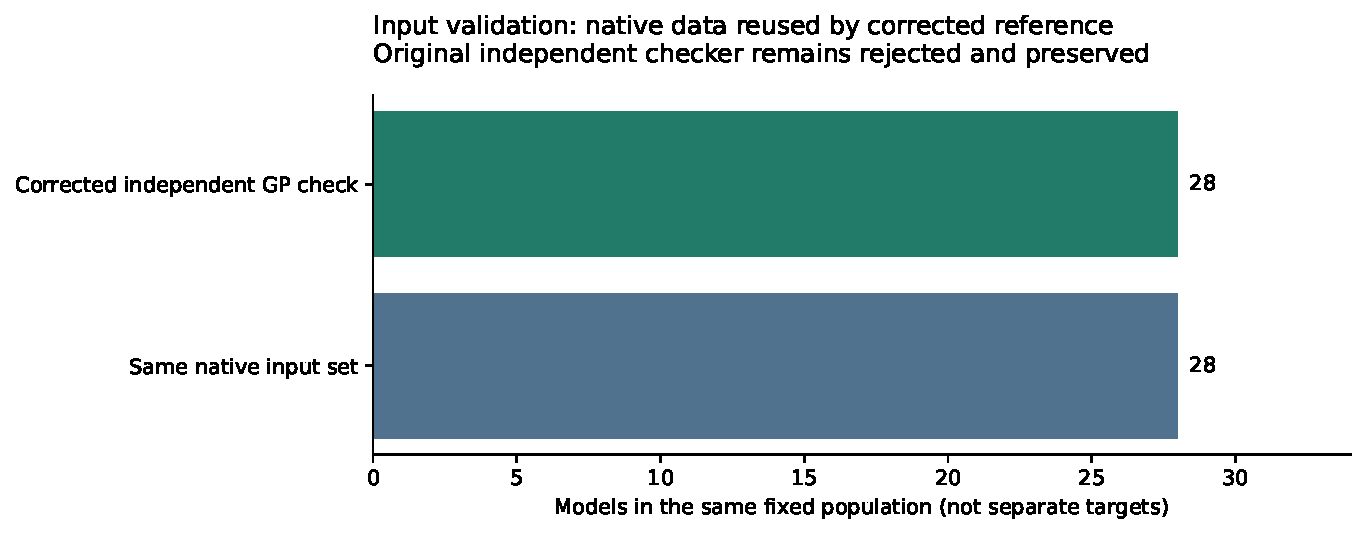
\includegraphics{INPUTS.pdf}
\caption{The same input population checked by two paths}
\end{figure}

Raw evidence: \href{../../execution-v15/.artifacts.json}{manifest},
\href{../../execution-v15/RAW_VERIFICATION.json}{all15 member hashes and
fresh repack check},
\href{../../execution-v15/reference-v2/experiment.export.v2.json}{corrected
export}.

Reproduction and raw-object manifests are linked from the evidence
directory. The user-confirmed store is
\texttt{setec-astronomy-artifacts}, region us-east-2. No NIST,
asymptotic, novelty or calibrated-GAE result is established.

\end{document}
